%%%%%%%%%%%%%%%%%%%%%%%%%%%%%%%%%%%%%%%%%%%%%%%%%%%%%%%%%%%%%%%%%%%%%%%%%%%%
%                                                                          %
%                                 PREAMBLE                                 %
%                                                                          %
%%%%%%%%%%%%%%%%%%%%%%%%%%%%%%%%%%%%%%%%%%%%%%%%%%%%%%%%%%%%%%%%%%%%%%%%%%%%
%\documentclass[confrence]{IEEEtran}
\documentclass[draftcls,onecolumn]{IEEEtran}
%%%%%%%%%%%%%%%%%%%%%%%%%%%%%%%%%%%%%%%%%%%%%%%%%%%%%%%%%%%%%%%%%%%%%%%%%%%
%                                                                         %
%                                 PREAMBLE                                %
%                                                                         %
%%%%%%%%%%%%%%%%%%%%%%%%%%%%%%%%%%%%%%%%%%%%%%%%%%%%%%%%%%%%%%%%%%%%%%%%%%%

%% PACKAGES
\usepackage[]{lineno}
%\linenumbers
\usepackage[usenames,dvipsnames]{xcolor}
\usepackage{microtype}
\usepackage[obeyDraft]{todonotes}
\usepackage{fancyvrb}
\VerbatimFootnotes
\usepackage{algorithmic}

%% GRAPHICS RELATED
\usepackage{graphicx}
\usepackage[outdir=./tmp/]{epstopdf}
\graphicspath{{../images/}{./}{./tmp/}}
\DeclareGraphicsExtensions{.eps, .pdf, .jpeg, .png,}

%% CPATION SETUP
\usepackage{float}
\usepackage{caption}
\usepackage{subcaption}
\captionsetup{belowskip=12pt,aboveskip=4pt}


%% BIBLIOGRAPHY
\bibliographystyle{ieeetr}

%% UNITS
\usepackage{siunitx}

%% EQUATIONS
\usepackage{amsmath}
%\numberwithin{equation}{section}

%% HYPERLINKS
\usepackage[debug]{hyperref}

%%%%%%%%%%%%%%%%%%%%%%%%%%%%%%%%%%%%%%%%%%%%%%%%%%%%%%%%%%%%%%%%%%%%%%%%%%%
%                                                                         %
%                             Listing Setup                               %
%                                                                         %
%%%%%%%%%%%%%%%%%%%%%%%%%%%%%%%%%%%%%%%%%%%%%%%%%%%%%%%%%%%%%%%%%%%%%%%%%%%
\usepackage{listings}
\lstset{ %
    language=C++,
    basicstyle=\footnotesize\ttfamily,
    numbers=left,
    numberstyle=\tiny\color{gray},
    stepnumber=2,
    numbersep=5pt,
    backgroundcolor=\color{white},
    showspaces=false,
    showstringspaces=false,
    showtabs=false,
    frame=single,
    rulecolor=\color{black},
    tabsize=2,
    breaklines=true,
    breakatwhitespace=false,
    title=\lstname,
    keywordstyle=\color{blue},
    commentstyle=\color{OliveGreen},
    stringstyle=\color{orange}
}
\DeclareCaptionFont{white}{\color{white}}
\DeclareCaptionFormat{listing}{\colorbox[cmyk]{0.43, 0.35, 0.35, 0.01}{\parbox{\dimexpr\textwidth-2\fboxsep\relax}{#1#2#3}}}
\captionsetup[lstlisting]{format=listing,labelfont=white,textfont=white,singlelinecheck=false,margin=0pt,font={bf,footnotesize}}
%\lstnewenvironment{code}[1][]%
%{ \noindent\minipage{\linewidth}
%	\lstset{#1}
%}
%{\endminipage}
%% USER COMMANDS
\usepackage{isotope}
\newcommand{\iso}{\isotope}
\newcommand{\figurewidth}{\textwidth}
\newcommand{\micron}{$\mu$m}


\DeclareSIUnit\roetgen{R}
\DeclareSIUnit\eV{\electronVolt}
\DeclareSIUnit\count{count}
\DeclareSIUnit\cps{\count\per\second}
\DeclareSIUnit\cpsngcf{\count\per\second\per\nano\gram\iso[252]{Cf}}
%%%%%%%%%%%%%%%%%%%%%%%%%%%%%%%%%%%%%%%%%%%%%%%%%%%%%%%%%%%%%%%%%%%%%%%%%%%%
%                                                                          %
%                               START OF DOCUMENT                          %
%                                                                          %
%%%%%%%%%%%%%%%%%%%%%%%%%%%%%%%%%%%%%%%%%%%%%%%%%%%%%%%%%%%%%%%%%%%%%%%%%%%%

\begin{document}
\title{Energy deposition in thin polymeric films}
\author{
    \IEEEauthorblockN{L.F. Miller\IEEEauthorrefmark{1}, M. J. Urffer\IEEEauthorrefmark{1}, A. Mabe\IEEEauthorrefmark{2}}
    \\
    \IEEEauthorblockA{\IEEEauthorrefmark{1}
    University of Tennessee \\
    Deparment of Nuclear Engineering \\
    Knoxville, Tennessee, 37916 \\
    }
    \IEEEauthorblockA{\IEEEauthorrefmark{2}
    University of Tennessee \\
    Deparment of Chemistry \\
    Knoxville, Tennessee, 37916 \\
    }
}

\maketitle

\begin{abstract}

Alternative neutron detection technologies are required to replace the current \iso[3]{He} based Radiation Portal Monitors (RPMs).
Pacific Northwest National Lab in conjuncation with the Department of Homeland Security had determined replacement technology criteria; namely a neutron detection criteria and that the perfomance of the detector should not suffer in the the presence of a strong gamma field.
The difference in the energy deposition mechanics from a charge particle (from the fission products of a neutron interaction) and the Compton scattered electrons from a gamma interaction allows for the effective discrimination between neutrons and gammas based on energy deposition.
Polymeric films containing \iso{6}{LiF} ranging from \SI{15}{\um} to \SI{1}{\cm} where fabricated and tested for their neutron count rate above a lower level discriminator necessary to meet the gamma intrisinic efficiency set forth by PNNL.
The energy deposition in the films was also simulated with GEANT4 and compared to the measured pulse height spectra.
\end{abstract}

\IEEEpeerreviewmaketitle

%%%%%%%%%%%%%%%%%%%%%%%%%%%%%%%%%%%%%%%%%%%%%%%%%%%%%%%%%%%%%%%%%%%%%%%%%%%
%                                                                         %
%                               INTRODUCTION                              %
%                                                                         %
%%%%%%%%%%%%%%%%%%%%%%%%%%%%%%%%%%%%%%%%%%%%%%%%%%%%%%%%%%%%%%%%%%%%%%%%%%%
\section{Introduction}
\label{sec:Intro}
The Department of Homeland Security (DHS) continues to fund research (through the Domestic Nuclear Detection Office (DNDO)) to detect radioactive material that could potentially be used to cause significant economic loss and loss or life.  
The current technology used in Radiation Portal Monitors (RPMs) for detections emitted from special nuclear material uses a rapidly diminishing resource, \iso[3]{He}, that cannot be economically replaced. 
As a result a number of alternative detection systems continue to be investigated with the most viable including: boron triflouride  filled proportional detectors, boron-lined proportional detectors, lithium-6 (\iso[6]{6}) loaded scintillation glass fiber detectors, and \iso[6]{Li} plus scintillator-coated wavelength-shifting fiber detectors\cite{kouzes_neutron_2010}.  

Replacement detection technologies must satisify a neutron detection efficiency while being insenstive to a given gamma field.
PNNL along with the DNDO have determined a set of specifications that that replacement RPMs must meet \cite{kouzes_neutron_2010, kouzes_neutron_1999}. 
The specifications consist of an absolute neutron detection efficiency greater than \SI{2.5}{\cps} at \SI{2}{\meter} for a defined moderated source, an intrinsic gamma-neutron detection efficiency of one in a million, and a gamma absolute rejection ratio for neutrons stating that the performance of the detector should not change by more than 10\% in a \SI{10}{\milli\roetgen\per\hour} gamma field.

%%%%%%%%%%%%%%%%%%%%%%%%%%%%%%%%%%%%%%%%%%%%%%%%%%%%%%%%%%%%%%%%%%%%%%%%%%%
%                                                                         %
%                                 THEORY                                  %
%                                                                         %
%%%%%%%%%%%%%%%%%%%%%%%%%%%%%%%%%%%%%%%%%%%%%%%%%%%%%%%%%%%%%%%%%%%%%%%%%%%
\section{Technical Basis}
The difference in the transfer of kinetic energy from charged particles to electrons and from photon interactions to electrons may be exploited to maximize discrimination between neutron and photon interactions in a detector.  
In particular, a photon interacts with a single electron and transfers a portion its energy to the electron predominately through Compton scattering. 
Neutron detectors often utilize a material with a large cross section for absorption, such as \iso[6]{li} or \iso[10]{B}.
When these materials absorb a neutron they usually disintegrate to produce ionized reaction products that in turn transfer their kinetic energy to many electrons.
The electrons from the neturon reation products generally have less energy than those from gamma interactions therefore depositing their energy in a shorter range.

For a particular material and neutron absorber, one can optimize the detector geometry to maximize the energy deposited in scintillation material by charged particles relative to the energy deposited by photon interactions. 
This in turn permits one to maximize the recorded neutron interaction rate relative to recorded photon interaction rates by setting a lower level discriminator (LLD) above a threshold associated with energy deposited in the detector by photons.  
As the LLD is increased, the efficiency for detecting neutrons is diminished; however, the intrinsic efficiency for detecting neutrons relative to photons is dramatically increased. 

%%%%%%%%%%%%%%%%%%%%%%%%%%%%%%%%%%%%%%%%%%%%%%%%%%%%%%%%%%%%%%%%%%%%%%%%%%%
%                                                                         %
%                                   METHODS                               %
%                                                                         %
%%%%%%%%%%%%%%%%%%%%%%%%%%%%%%%%%%%%%%%%%%%%%%%%%%%%%%%%%%%%%%%%%%%%%%%%%%%
\section{Methods}
\label{sec:Methods}
The energy deposition of neutrons and gammas was investigated for polymeric films containing \iso{Li}{6} as \iso{LiF}{6} of thickness ranging from \SI{15}{\um} to \SI{1}{\cm}.
The pulse height spectra of these samples was measured on site at the University of Tennessee's characterization laboratory from a moderated neutron source as wells as a \iso{Co}{6} source.
Simulations were completed using GEANT4, a modern toolkit for Monte Carlo transport simulation \cite{agostinelli_geant4simulation_2003,allison_geant4_2006}.
The measurements were then used to validate and bench marking the simulation.

\subsection{Fabricated Detector Measurements}
Samples are mounted to a 10 stage PMT with silicone based optical grease. 
The PMT is attached to a Canberra base (also serving as a preamplifier). 
The PMT's voltage is supplied by a high voltage power supply, with the power being supplied to the pre amplifier base by an amplifier.  
The output signal of the base feeds into the amplifier for pulse shaping and amplification. 
The amplified signal is then inputted to an MCB-ADC, and can then be read using the MAESTRO-32 software. 
A schematic of the setup is shown in Figure ~\ref{fig:ElectronicsSpectra}.
\begin{figure}
	\centering
	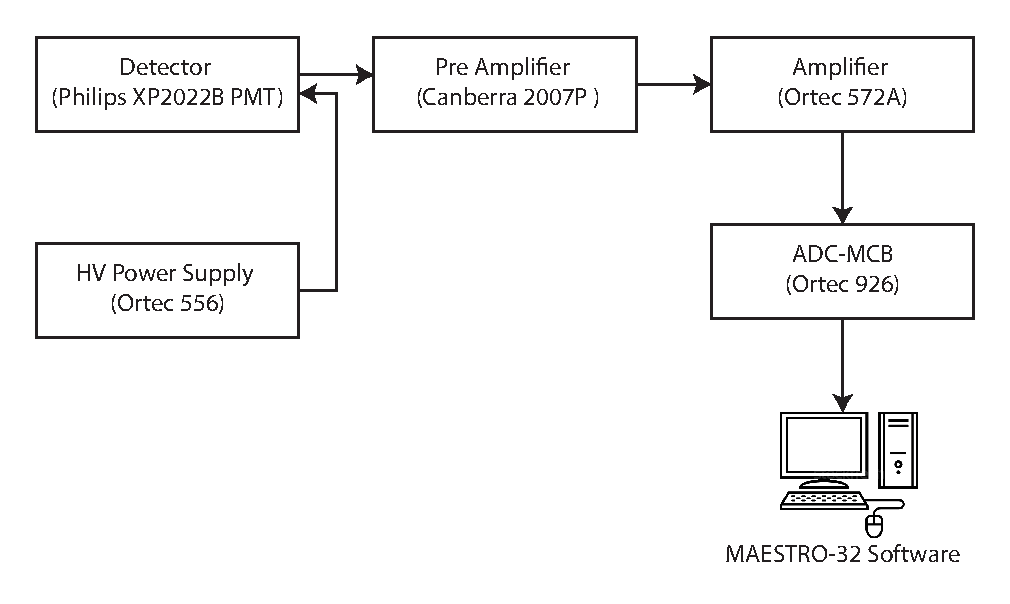
\includegraphics[width=\figurewidth]{ElectronicsSpectra}
	\caption{Pulse height measurement electronics}
	\label{fig:ElectronicsSpectra}
\end{figure}

 The films where exposed to a 100 $\mu$Ci \iso{60}{Co} source producing a \SI{10}{\milli\roetgen\per\hour} field. 
The gamma irradiator is a thin steel outer box 14” x 12” x 12” which contains 4” x 8” x 2” lead bricks.  
The 100 $\mu$Ci \iso{60}{Co} source is contained in 2” of steel, with a 1/8” thick steel cap.  
The detector well is a 4” outer diameter 14” pipe that is ¼” thick, and \SI{7}{\cm} of foam is used to ensure that the detector rests at a \SI{10}{\milli\roetgen\per\hour} field. 
Figure ~\ref{fig:gammaIrridiator} shows an MCNPX rendering of the gamma irridiator.
\begin{figure}
	\centering
	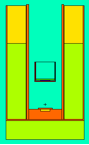
\includegraphics[width=\figurewidth]{GammaIrridiatorMCNPXRender.png}
	\caption{MCNPX Rendering of Gamma Irridiator}
	\label{fig:gammaIrridiator}
\end{figure}
The gamma intrinsic efficiency of the sample is calculated by integrating the mesured spectra, $p(x)$, as a function of a mathmatical lower level channel discrimiantor ($MLLD$) setting and dividing by the incident photon fluence, $\Phi$, as shown in \eqref{eqn:mlld}.
The incident photon fluence was calculated with MCNPX and confirmed by measurments.
\begin{align}
	\label{eqn:mlld}
	\epsilon_{int,\gamma} \left(MLLD\right) = \frac{\int_{MLLD}^\infty p(x)dx}{\Phi} 
\end{align}
The intrisinic effieciency of one in a million, $\epsilon_{int,\gamma} \le \si{1E-6}$, is determined by the $MLLD$ (corresponding to a channel) for which $\epsilon_{int,\gamma} \left(MLLD\right) \le \si{1E-6}$.

A moderated \iso{Cf}{252} source is used to measure the neutron spectra.
The neutron irradiator is a custom built \SI{0.59}{\ug}\iso[252]{Cf} source encased in 2” blocks of high density polyethylene (HDPE).
The HDPE box is approximately 20” long, 12” wide, and 14” tall (Figure 6).
There are two detector 1/16” thick acrylic detectors wells, one surrounded by a 1/16” cadmium to shield out thermal neutrons, and the other surrounded by 1/16” of lead to shield out a similar amount of gammas as the cadmium well.
The \SI{0.59}{\ug}\iso[252]{Cf} source is surrounded by stainless steel, which in turn is contained within a 2” diameter, ½” thick, 5 ¼” tall lead vessel. 
Figure ~\ref{fig:neturonIrridiator} is an MCNPX rendering of the neutron irridiator.
\begin{figure}
	\centering
	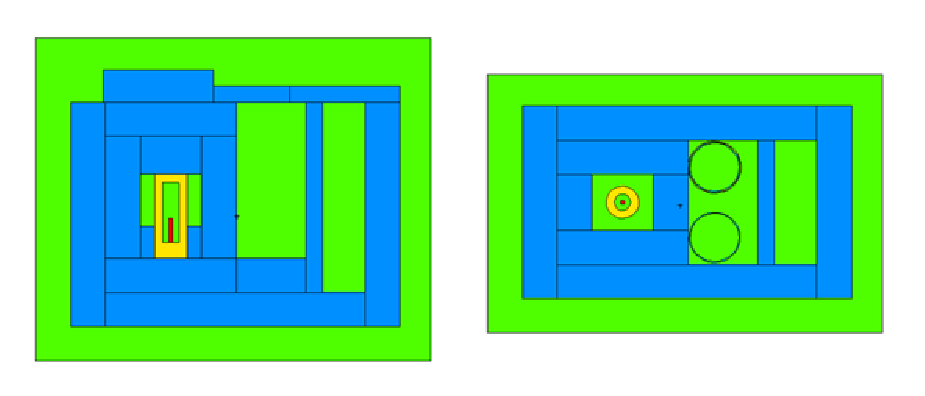
\includegraphics[width=\figurewidth]{NeutronIrridiator_MCNP.eps}
	\caption{MCNPX Rendering of Neutron Irridiator}
	\label{fig:neutronIrridiator}
\end{figure}
The lead well measures the response of neutron of all energies, while the cadmium well measures the responses of fast neutrons.
The two responses are then subtracted to yeild the thermal neutron response.

While this source is not the same configuration as specified by PNNL, neutronic simulations in MCNPX can be used to relate the interactions to a simulated interaction rate for a detector mocked up according the the PNNL specifications encased in the RPM8 footprint.

\subsection{Detector Simulation}
The energy deposition from neutron and gamma interactions was simulated with the GEANT4 toolkit \cite{agostinelli_geatn4simulation_2003}.
The detector geometry was represented as a single layer of neutron absorbing material mounted atop of a non-scintillating material (PMMA).
The initial events for runs where chosen by setting up a particle gun for thermal (0.025 eV) neutrons upon the detector and for both gammas resulting from a \iso{Co}{60} decay.
The Livermore physics were used as the ionization module, extending the standard electro-magentic physics down to \SI{250}{\eV}, and a micro dose model, G4DNAPysics, was used to transport the electrons down to \SI{10}{\eV}.
High performance, data driven hadronic modules were used in order to simulate the neutron and the subsquenet reaction product transport.

The simulation was validated by reproducing the single collision energy loss for water as well as comparing spectra shapes and averages of simulated spectra to the measured spectra.
The single collision energy loss spectra for water that was simulated is shown in Figure ~\ref{fig:SingleCollisionELossWater}.
In general there was excellent agreement between the simulated energy spectra and a previously published spectra\cite{turner_comparative_1982}, with the simulated spectra having much better resolution at fine energies (corresponding to discrete states) of which the reference did not.
It is thought that this is due to the water model in GEANT4 having better cross sections than the previously published spectra.
\begin{figure}[h]
    \centering
    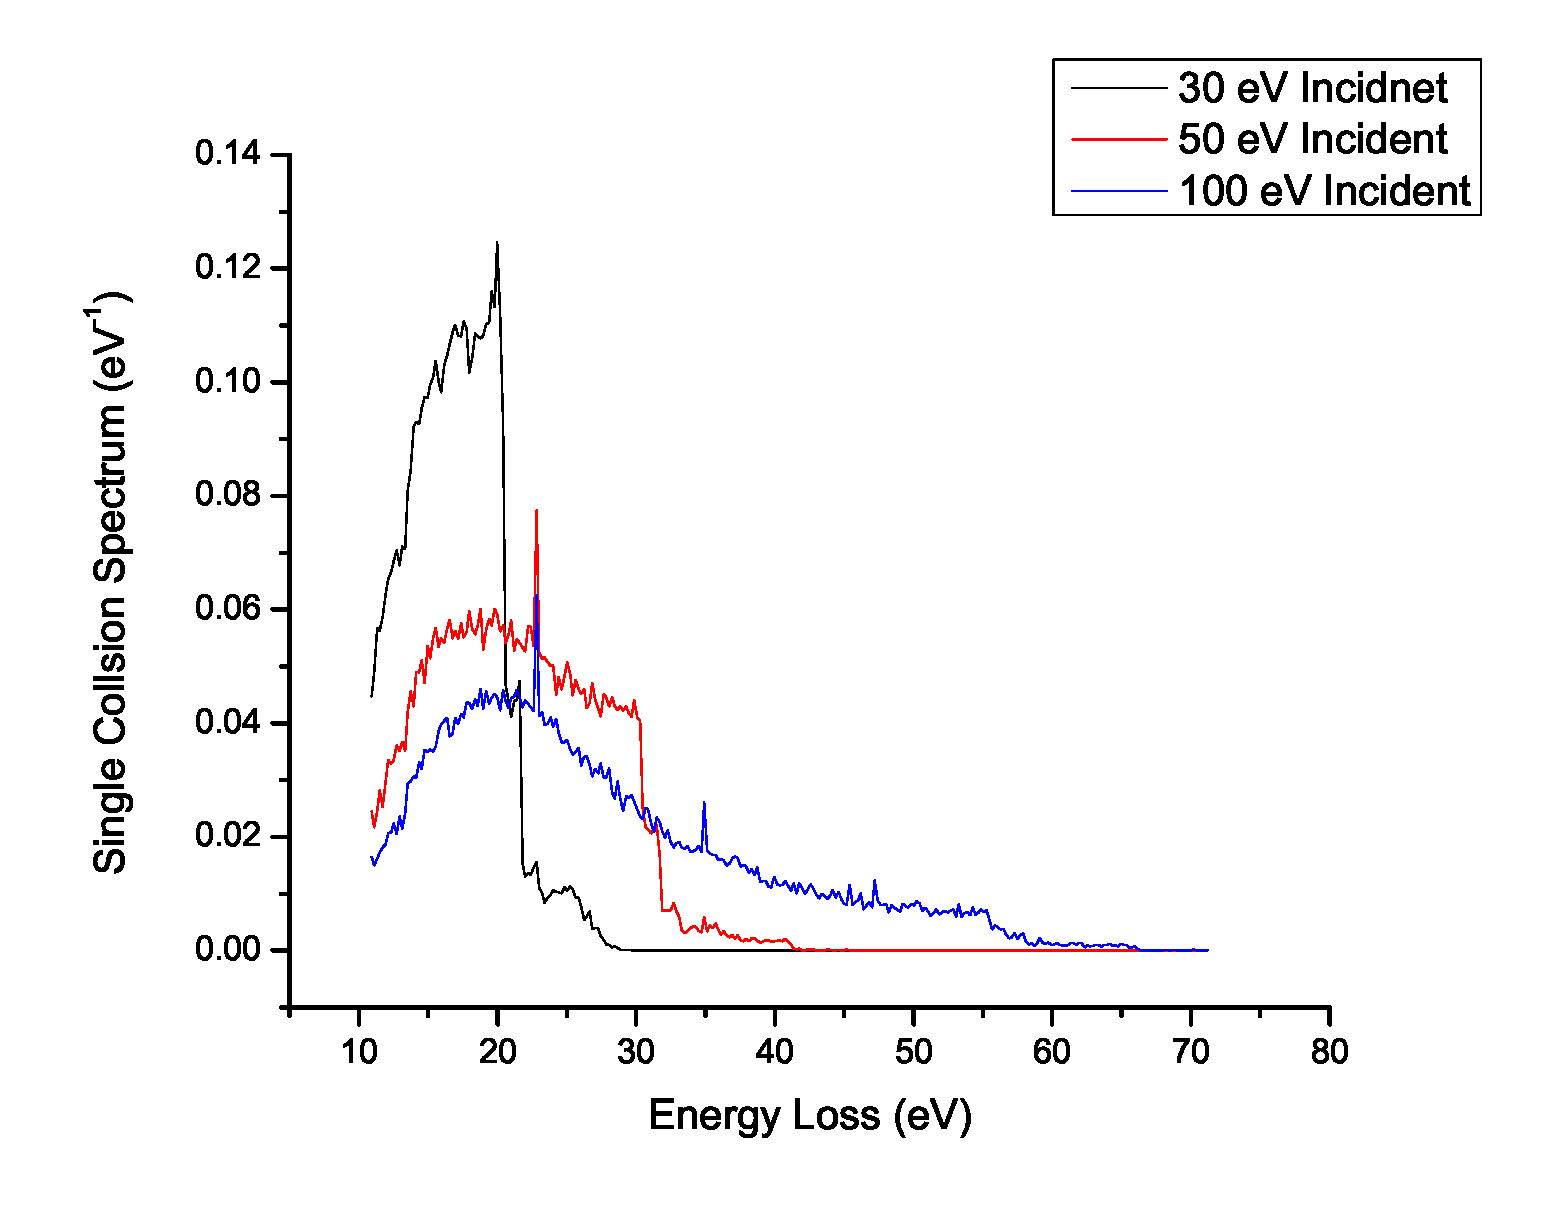
\includegraphics[width=\textwidth]{SingleCollisionEnergyLoss_300bins}
    \caption{Single Collision Energy Loss of Water}
	\label{fig:SingleCollsionELossWater}
\end{figure}

It is well established that the pulse height of a radiation event is proportional to the energy deposition of the event\cite{birks_scintillations_1951}.
Thus, the validity of the GEANT4 simulation can be determined by comparing the spectra shapes of measured spectra to simulated energy deposition.
Figure ~\ref{fig:spectraComparisonGamma} shows the comparison between the simulated energy depostion from a \iso[60]{Co} source and the measured pulse height spectra from the \iso[60]{Co} irridiator.

\begin{figure*}[h]
	\centering
	\begin{subfigure}[b]{0.45\figurewidth}
    		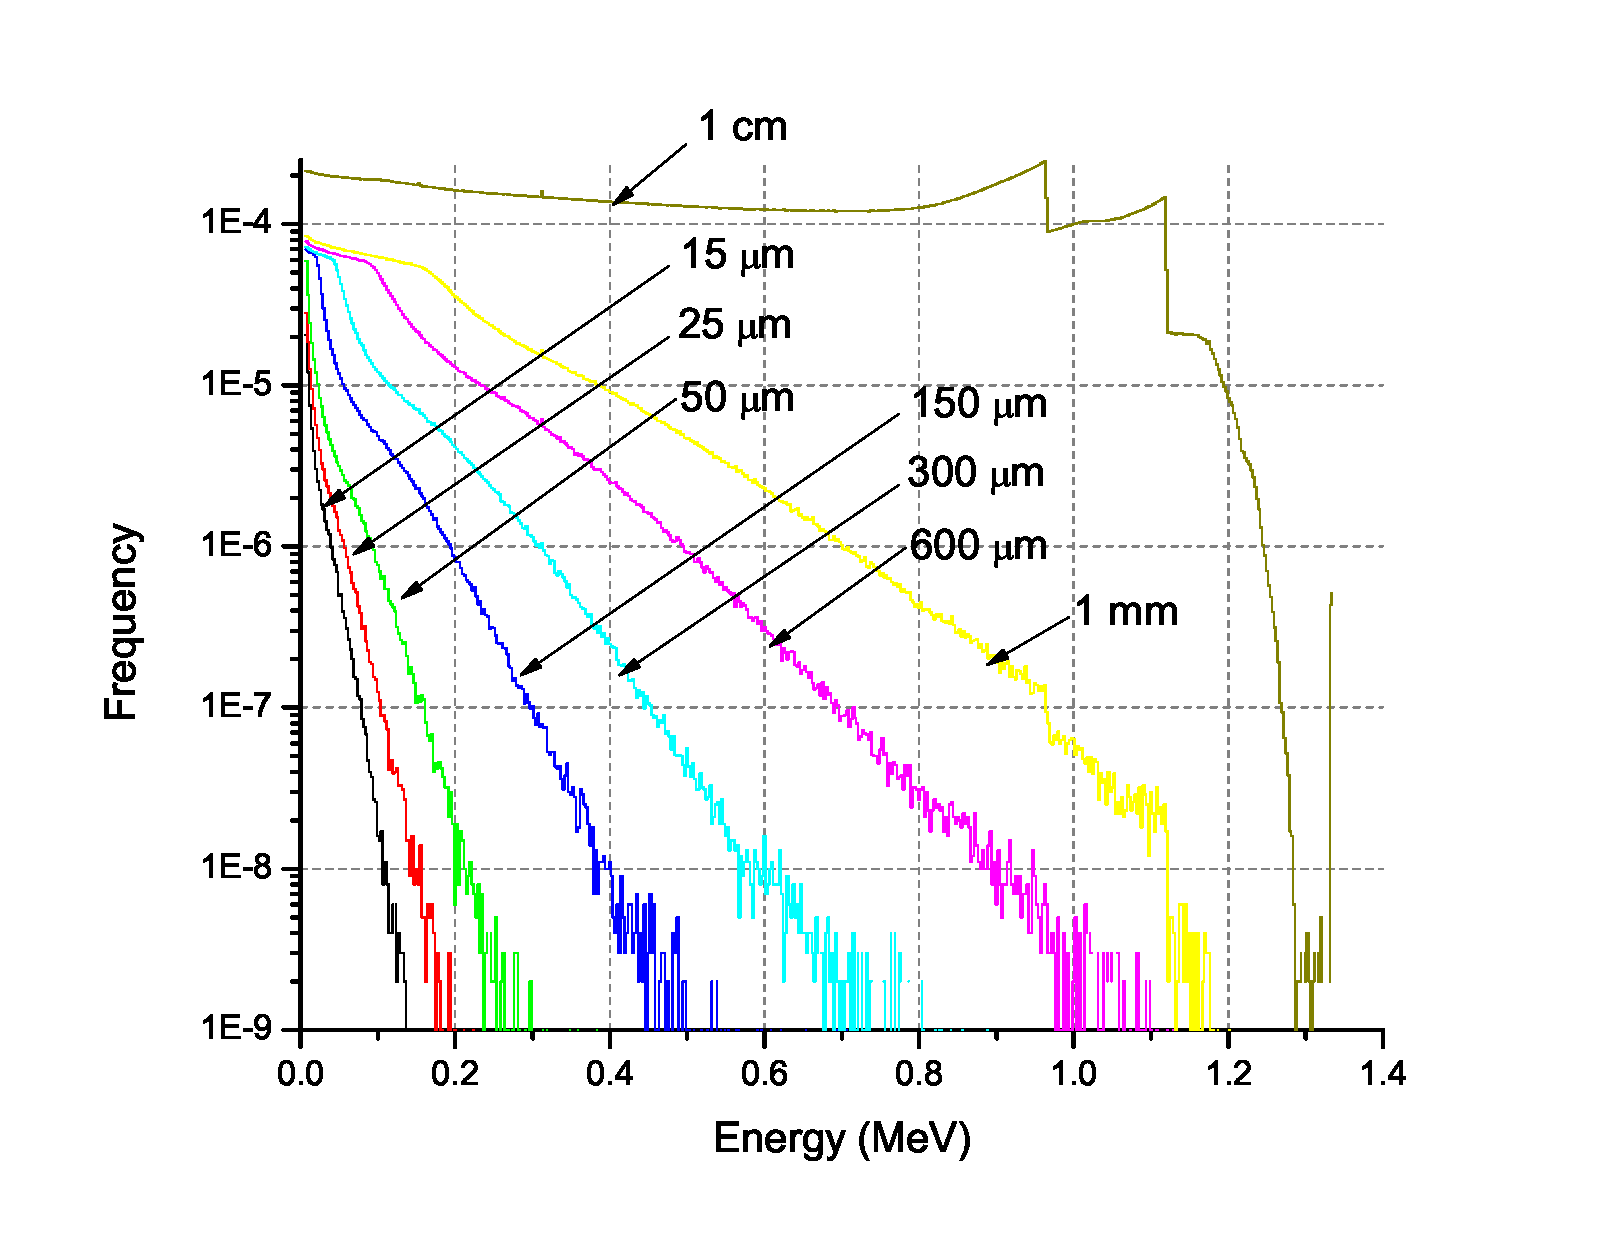
\includegraphics[width=\textwidth]{PS_EDepSim_Co60}
		\caption{Simulated Energy Depositon}
	\end{subfigure}%
	~
	\begin{subfigure}[b]{0.45\figurewidth}
    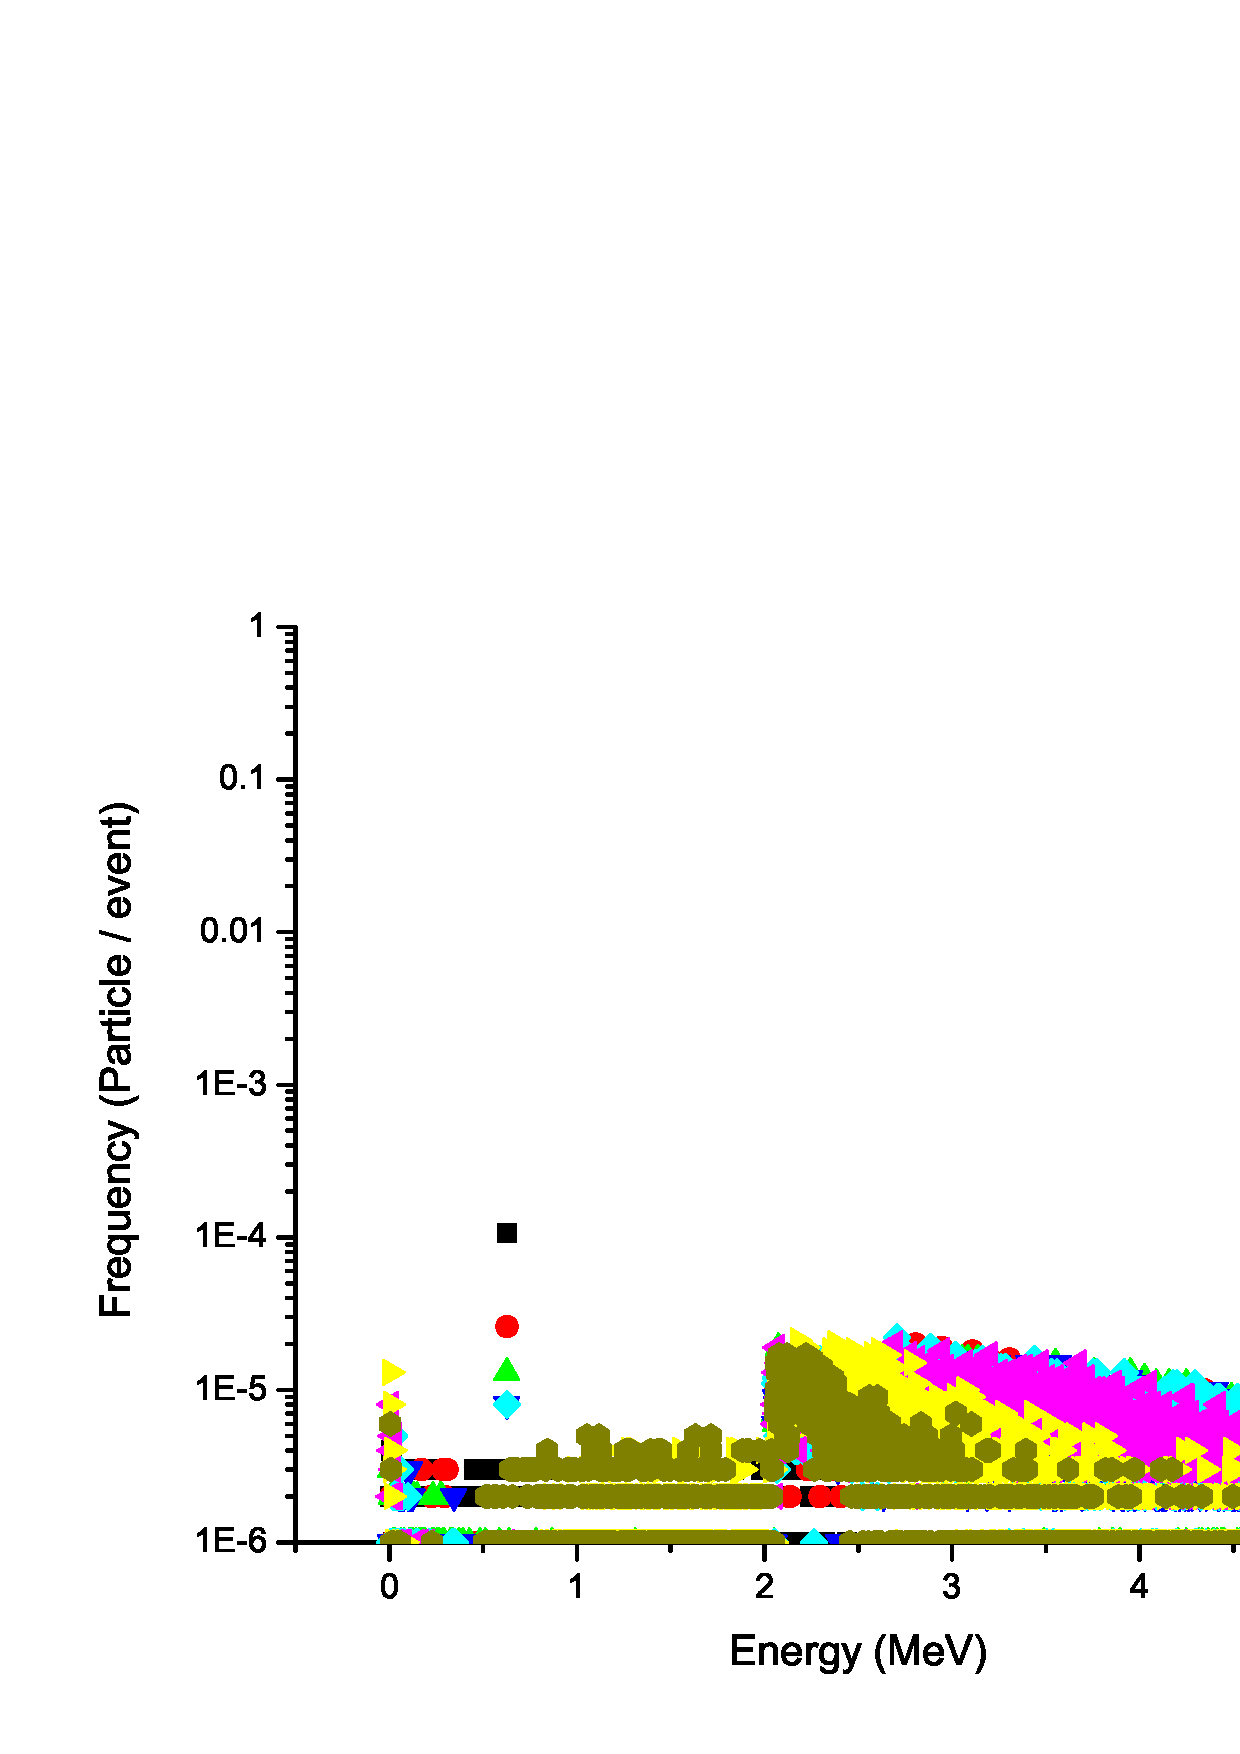
\includegraphics[width=\textwidth]{PS_EDepSim_Neutron}
		\caption{Measured Pulse Height Spectra}
	\end{subfigure}%
	\caption{Comparison of the energy deposition and pulse height spectra for validation. The spectra have the same shape, indicating agreement.}
	\label{fig:SimEDepGamma}
\end{figure*}
A more quantitative approach was taken for validation by computing the average energy deposition and pulse height, the results of which are shown in Figure ~\ref{fig:EDepLightYield}. 
With the average energy deposition on the left axis and the average light yield (pulse height) on the right axis, it is possible to compare the measurement and the simulation and agreement is observed.
\begin{figure*}[!ht]
	\centering
	\begin{subfigure}[b]{0.45\figurewidth}
    		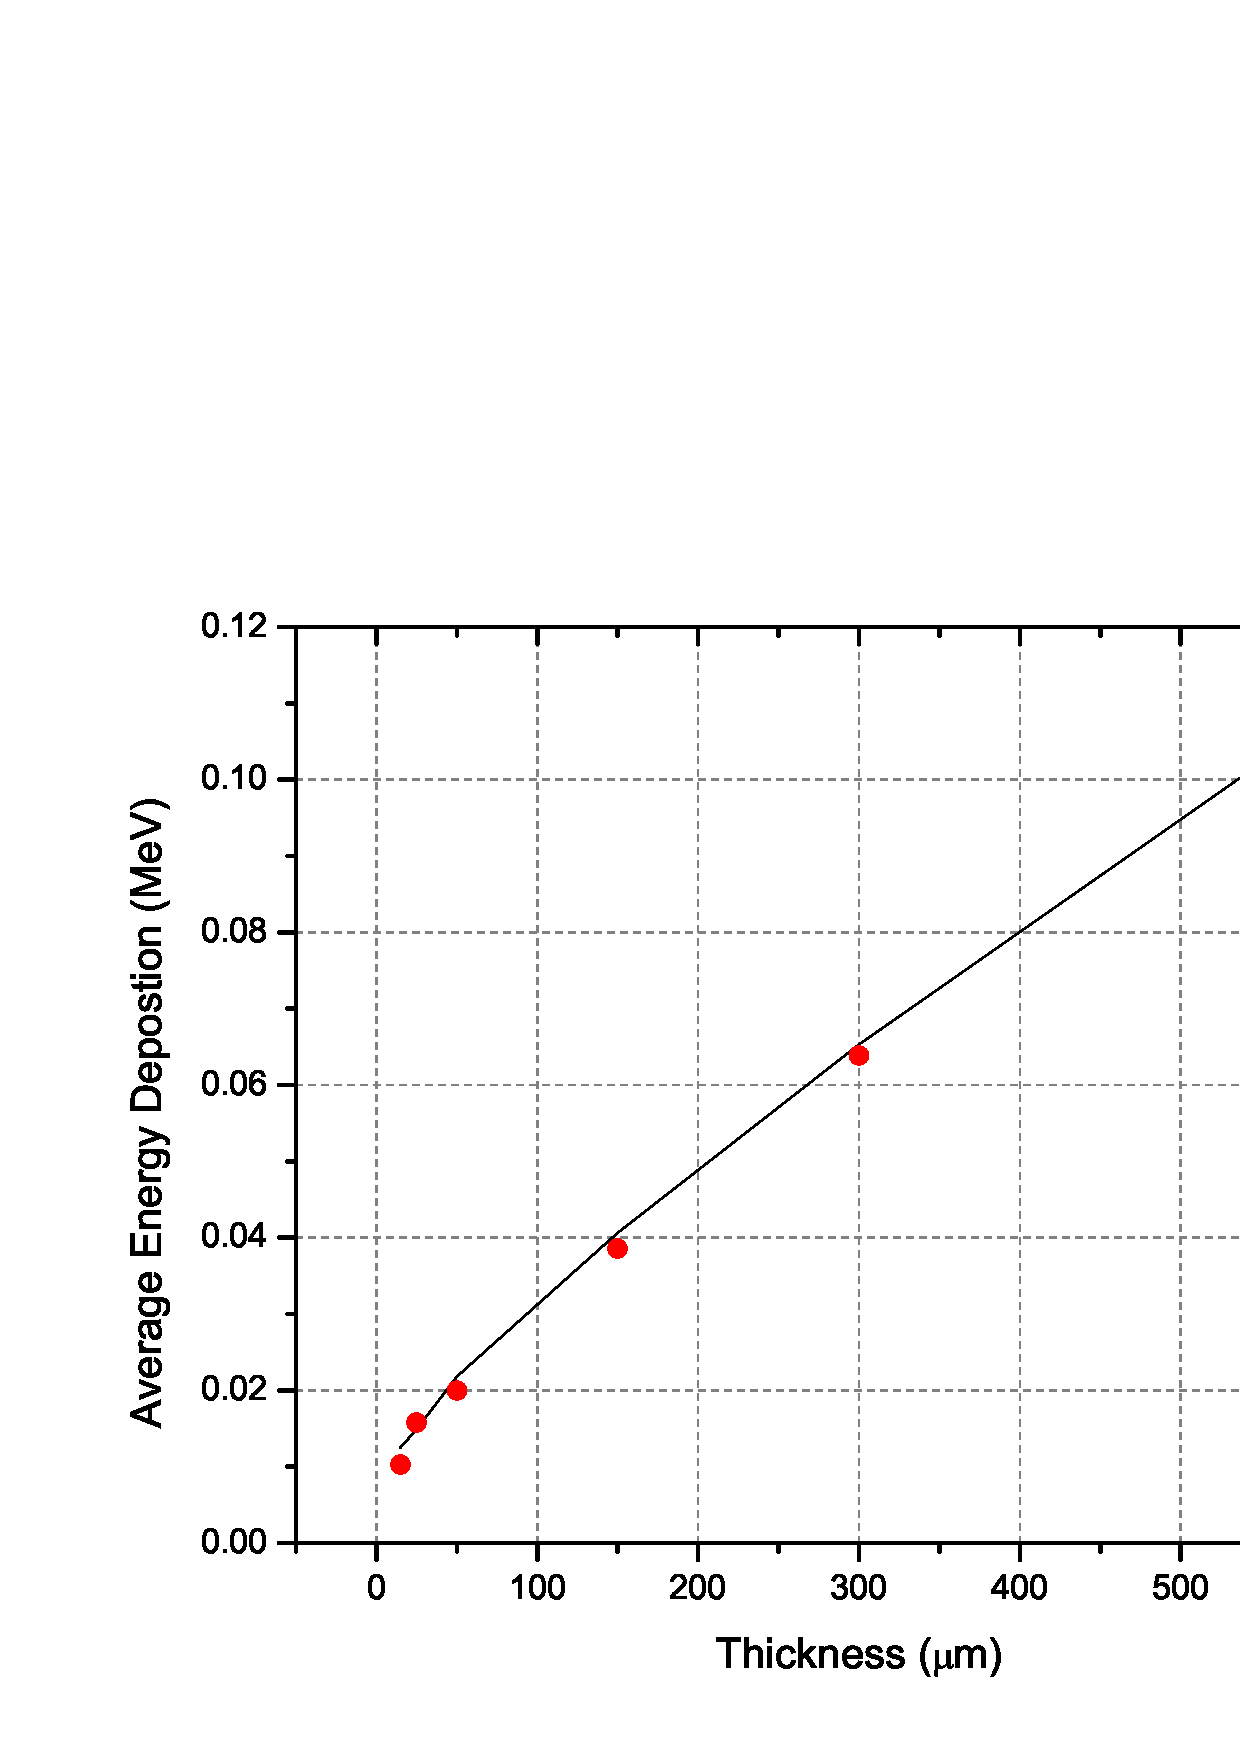
\includegraphics[width=\textwidth]{G4EDep_LightYield_Co60}
		\caption{Gamma (\iso{Co}{60})}
	\end{subfigure}%
	~
	\begin{subfigure}[b]{0.45\figurewidth}
    		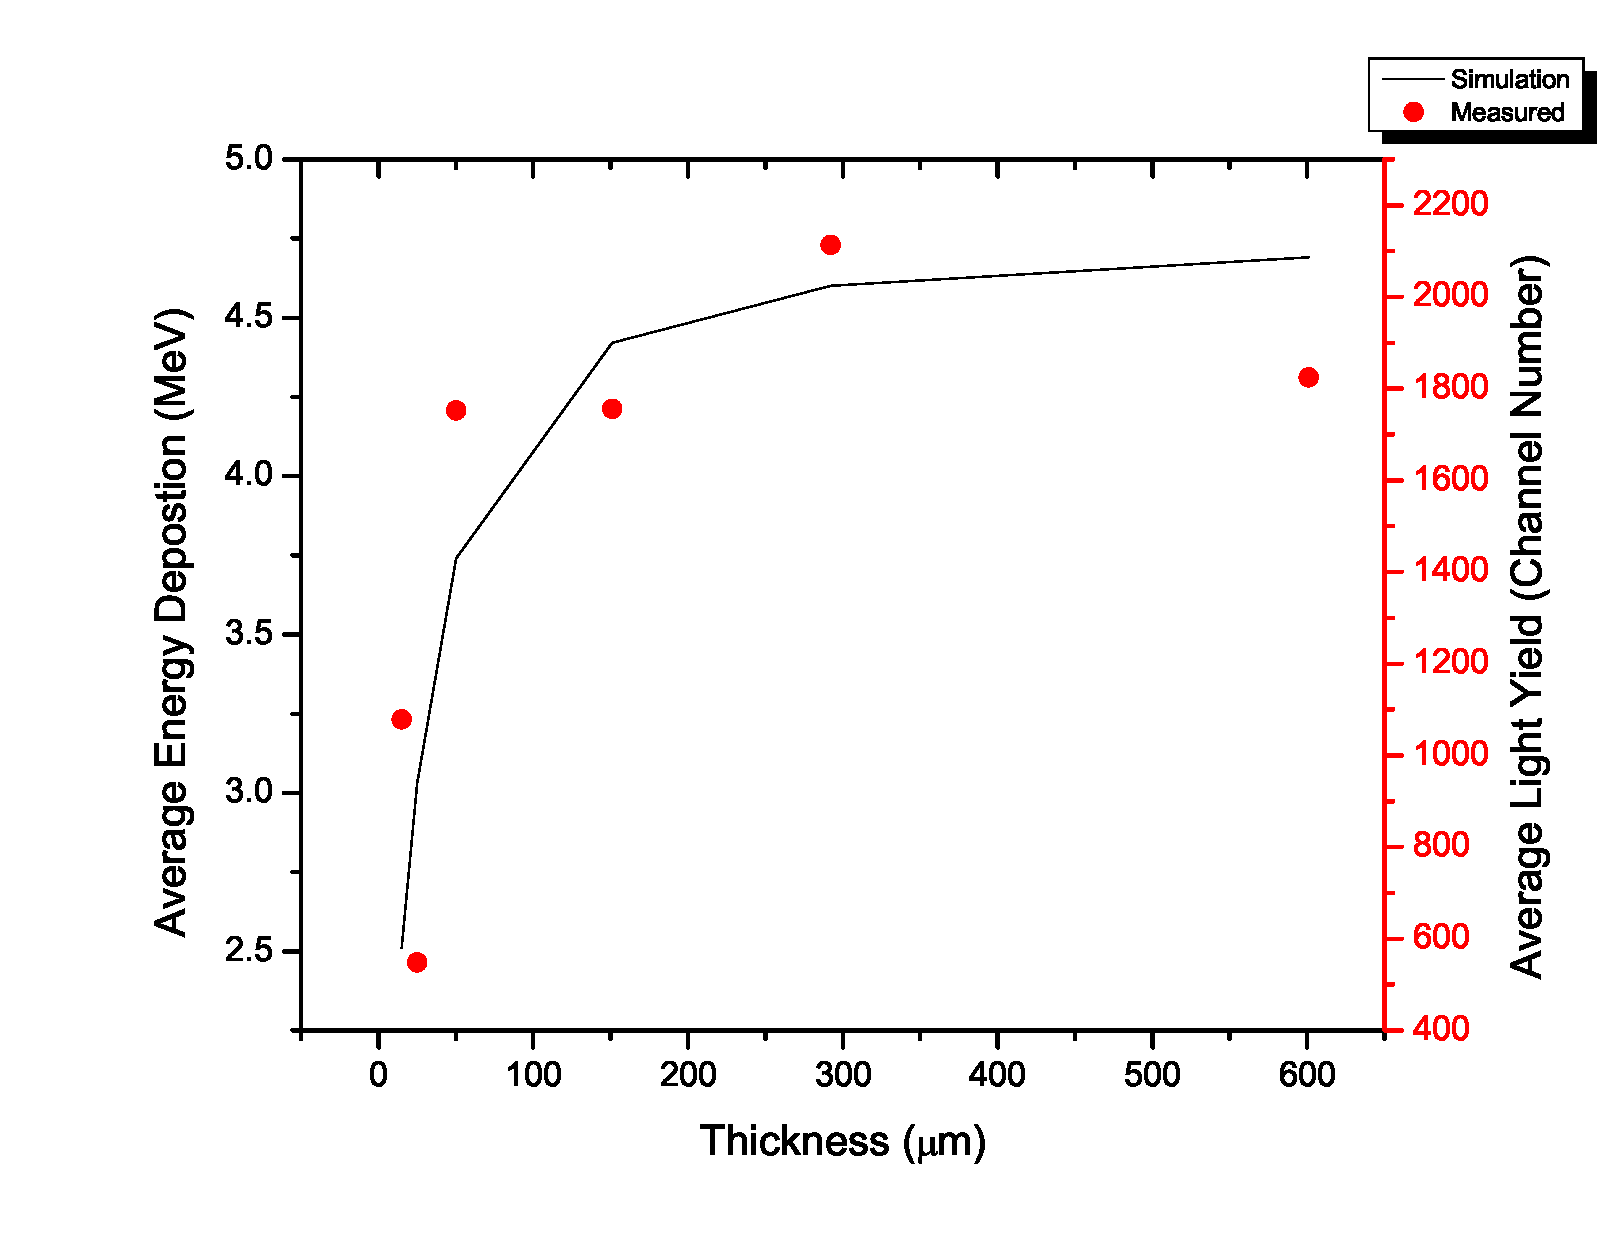
\includegraphics[width=\textwidth]{G4EDep_LightYield_Neutron}
		\caption{Neutrons}
	\end{subfigure}%
	\caption{Average Energy Deposition and Measured Light Yield}
	\label{fig:EDepLightYield}
\end{figure*}
%%%%%%%%%%%%%%%%%%%%%%%%%%%%%%%%%%%%%%%%%%%%%%%%%%%%%%%%%%%%%%%%%%%%%%%%%%%
%                                                                         %
%                     RESULTS and ANALYSIS                                %
%                                                                         %
%%%%%%%%%%%%%%%%%%%%%%%%%%%%%%%%%%%%%%%%%%%%%%%%%%%%%%%%%%%%%%%%%%%%%%%%%%%
\section{Results}
\label{sec:Results}
The calculated gamma intrisinic efficiency for six polymeric films along with the neutron response of two of the films in Figure ~\ref{fig:GammaIntrNeutronCounts}. 
It is observed that if the films are thin enough (less than \iso{150}{\um}) it is possible to have a significant count rate above the the mathmatical lower level discriminator necessary for the pulse height discrimination of one in a million.
\begin{figure}[h]
    \centering
    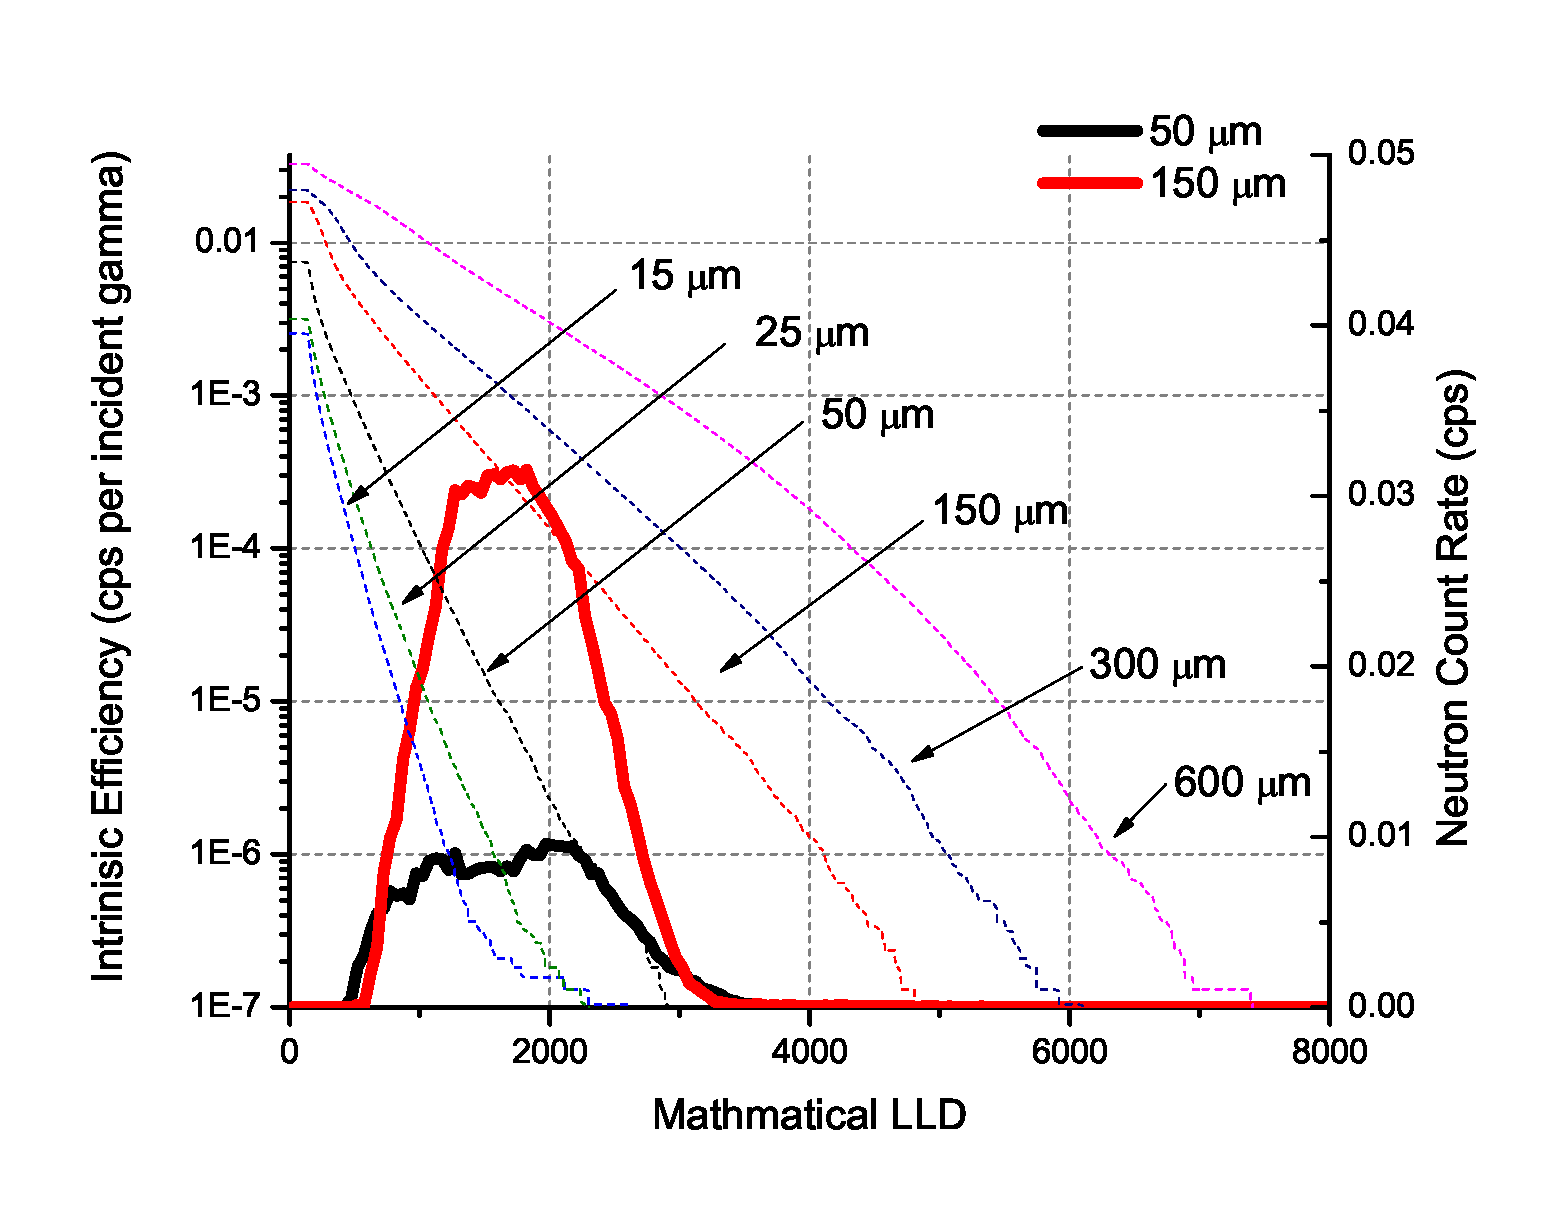
\includegraphics[width=\figurewidth]{PS_IntEff_LiF20_PPO5}
    \caption{Gamma intrinsic efficiency (dashed lines) plotted against neutron counts (solid). The gamma spectra has been normalized by the number of incident photons upon the sample, while the neutron spectra has not.}
    \label{fig:GammaIntrNeutronCounts}
\end{figure}
The fraction of neutron counts above the MLLD necessary for a given gamma intrisinic efficinecy is plotted in Figure ~\ref{fig:crVsIntEff}.
It is observed that films thinner than \SI{150}{\um} have a very much larger fraction of neutron counts above an intrisinic efficiency of 1 in a million.
\begin{figure}[h]
    \centering
    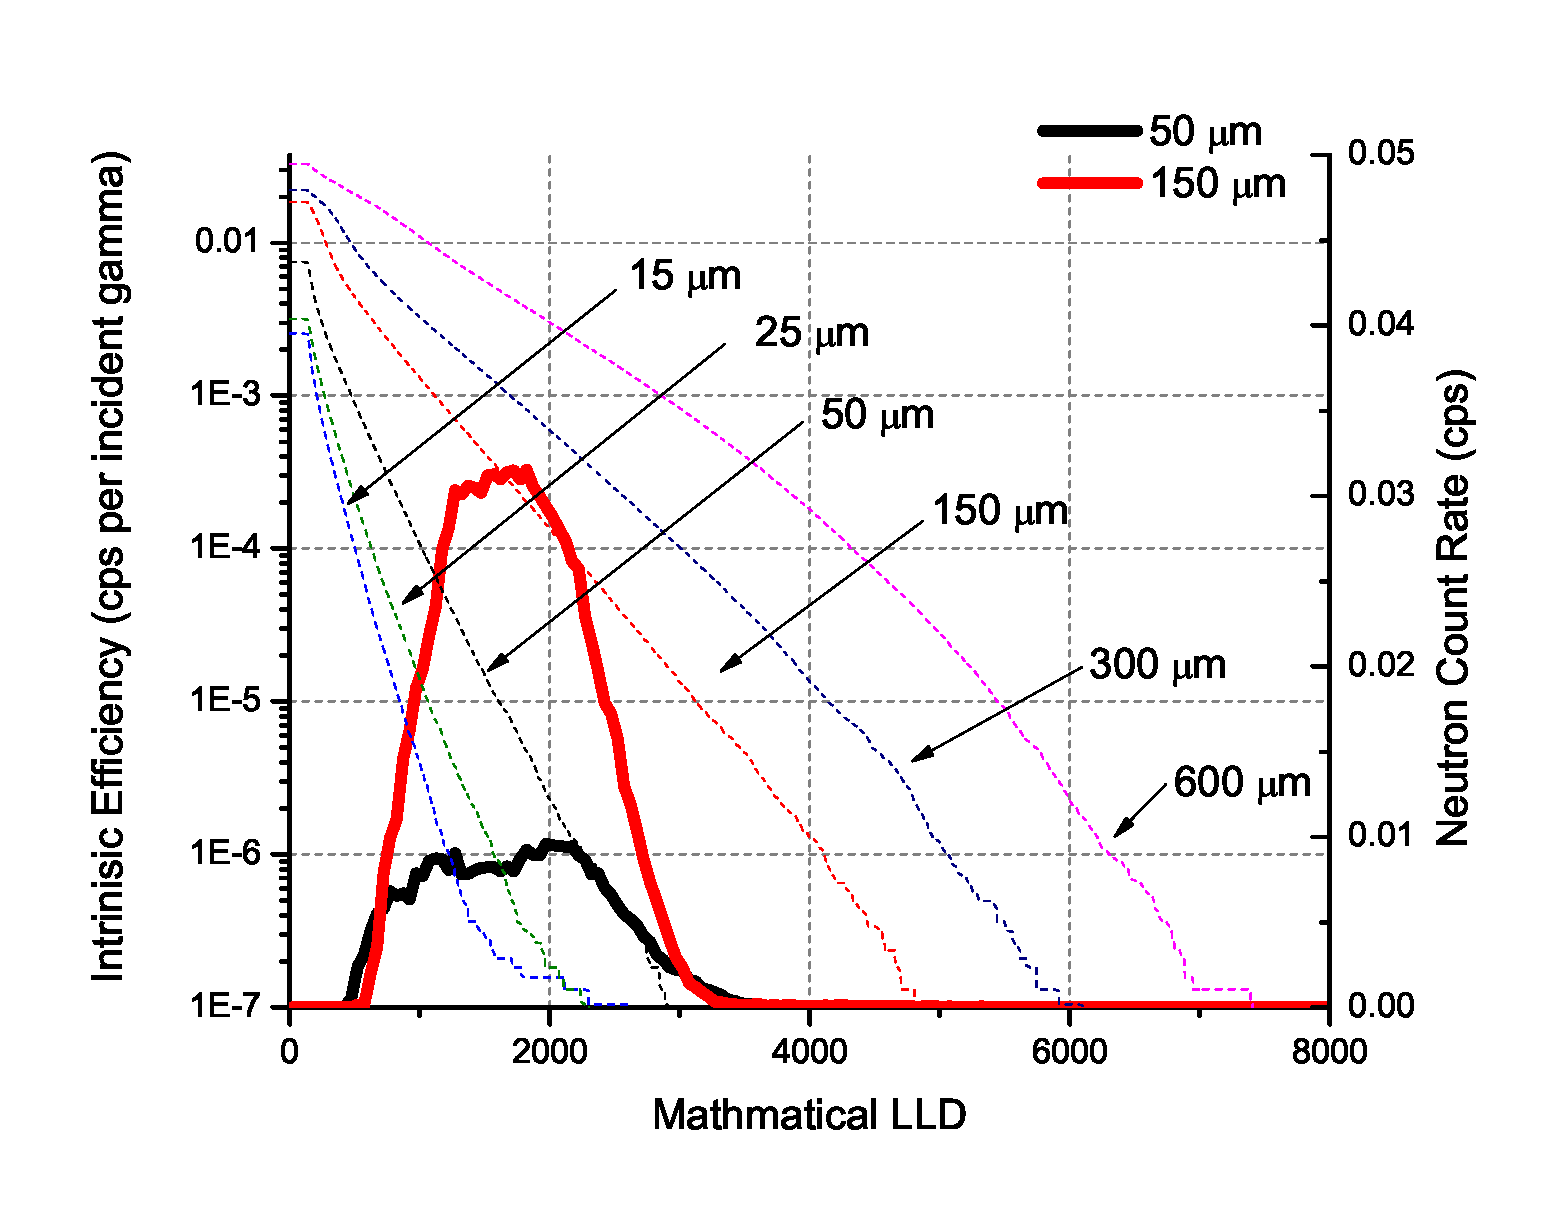
\includegraphics[width=\figurewidth]{PS_IntEff_LiF20_PPO5}
    \caption{Figure from pg. 7}
    \label{fig:crVsIntEff}
\end{figure}

The average energy deposited was computed for each thickness and and normalized by the incident energy for gammas or the Q-value of the reaction for neutrons, and is presented in Table ~\ref{tab:FractionEDep}.
\begin{table}[!htb]
    \caption{Fractional Energy Deposition for Various Thickness}
	\centering
	\begin{tabular}{c | c c}
	Thickness & Gamma Fraction & Neutron Fraction \\
	\hline
	\hline
	\SI{15{\um} & 0.010 & 0.531 \\
	\SI{25}{\um} & 0.013 & 0.634 \\
	\SI{50}{\um} & 0.017 & 0.782 \\
	\SI{150}{\um} & 0.032 & 0.927 \\
	\SI{300}{\um} & 0.052 & 0.964 \\
	\SI{600}{\um} & 0.087 & 0.982 \\
	\SI{1}{\mm} & 0.130 & 0.989 \\
	\SI{1}{\cm} & 0.425 & 0.998 \\
	\hline
	\end{tabular}
    \label{tab:FractionEDep}
\end{table}
For thickness greater than \SI{150}{\um} there is little benifit in increasing the thickness of the film in terms of energy deposition; already over 90\% of the energy is being deposited in the film.

%%%%%%%%%%%%%%%%%%%%%%%%%%%%%%%%%%%%%%%%%%%%%%%%%%%%%%%%%%%%%%%%%%%%%%%%%%%
%                                                                         %
%                             CONCLUSIONS                                 %
%                                                                         %
%%%%%%%%%%%%%%%%%%%%%%%%%%%%%%%%%%%%%%%%%%%%%%%%%%%%%%%%%%%%%%%%%%%%%%%%%%%
\section{Conclusions and Future Work}
\label{sec:Conclusions}

The question is how much energy deposition is required to make a photon?

The low interaction rate of the thins films suggest a layered detector detector design in order to increase the neutron interaction rate, provided that the layers are spaced by non-scintillating material of thickness greater than the maximum electron from a Compton scattering from \iso[60]{Co} (around \SI{5}{\mm}).
Future work will focus on the optimization of such a layered detector RPM.
In addition, light transport in layered thin film detectors will be explored.
%%%%%%%%%%%%%%%%%%%%%%%%%%%%%%%%%%%%%%%%%%%%%%%%%%%%%%%%%%%%%%%%%%%%%%%%%%%%
\section{Acknowledgments}
This works was supported by the Domestic Nuclear Detection Office (DNDO) through award 003387891.
Any opinions, findings, and conclusions or recommendations expressed in this material are those of the authors and do not necessarily reflect the views of DNDO.

% Bibliography
\bibliography{./Zotero}

\end{document}

